\chapter{Ionización de átomos y moléculas}
\label{chap:iondim}

En este Capítulo se estudia la estructura de átomos y moléculas pequeñas
a través de la ionización simple. La descripción de los blancos se 
obtiene a partir de potenciales efectivos que resultan de la 
implementación del método de inversión depurada. La efectividad de este 
método se examina a partir de su habilidad para describir la estructura 
de los blancos en el proceso colisional.

%%%%%%%%%%%%%%%%%%%%%%%%%%%%%%%%%%%%%%%%%%%%%%%%%%%%%%%%%%%%%%%%%%%%%%%%
\section{Introducción}
%%%%%%%%%%%%%%%%%%%%%%%%%%%%%%%%%%%%%%%%%%%%%%%%%%%%%%%%%%%%%%%%%%%%%%%%

%% Métodos para describir blancos
%%  - Estructura electrónica: HF, DFT 
%%  - Potenciales efectivos 
%%  - Potenciales de intercambio (Slater, OEP, etc)
%% Métodos para describir procesos colisionales
%%  - Born
%% Lo que se hizo en este trabajo
%%  - DIM en átomos
%%  - DIM en moléculas
%%  - FBA para ionización/fotoionización en atomos y moléculas simples

Las probabilidades de transición en una colisión inelástica se pueden 
obtener a partir de la correcta representación de los estados inicial y 
final del blanco. En general, la resolución de las ecuaciones de 
Schr\"odinger de sistemas multielectrónicos atómicos implementan el 
modelo de partículas independientes en conjunción con la aproximación 
de campo central~\cite{Bransden:03,Cowan:81}. Por ejemplo, el método de 
Hartree--Fock~(\acs{hf}) tiene a esta aproximación como hipótesis 
fundamental. Por otro lado, la descripción de la estructura electrónica 
de sistemas moleculares constituye un desafío desde el punto de vista 
teórico de primeros principios debido a su simetría no esférica y 
multicéntrica. Sin embargo, a lo largo del último siglo se han 
desarrollado diversas aproximaciones para tal 
fin~\cite{Helgaker:00,Schaefer:04}, siendo la más exitosa entre ellas la 
teoría del funcional de la densidad~(\acs{dft}, por sus siglas en 
inglés).

En un proceso colisional, la existencia de un potencial efectivo local 
que permita obtener de forma directa las funciones de onda de las 
partículas interactuantes es ideal. Con este fin, se han desarrollado 
diversas metodologías para el diseño de potenciales efectivos en blancos 
atómicos~\cite{Hibbert:82} y moleculares~\cite{Menchero:10,Granados:16}. 
Entre ellos se destacan algunos modelos 
paramétricos~\cite{Gombas:56,Green:69,Klapisch:71}, basados en el 
formalismo de HF~\cite{Phillips:59,Herman:63}, de polarización del 
núcleo electrónico~\cite{Dalgarno:70,Bayliss:77} y 
relativistas~\cite{Cowan:76,Lee:77}. Otra técnica conocida es la 
determinación de potenciales centrales a partir de funciones de onda y/o 
densidades electrónicas, llamada método de inversión. Este procedimiento 
ha sido estudiado de forma extensa en la DFT~\cite{Wu:03,Gaiduk:13,
Ryabinkin:15,Schipper:97,deSilva:12,Kananenka:13,Mura:97,Jacob:11}. En 
la teoría de colisiones, el método de inversión fue sugerido por Hilton 
\textit{et al.} en aplicaciones circunscriptas al cálculo de procesos de 
fotoionización en átomos~\cite{Hilton:77,Suzer:77}, agua~\cite{Hilton:79} 
y otras moléculas~\cite{Hilton:80,Crljen:87}. A su vez, estos trabajos 
se refieren a trabajos previos en polarizabilidad atómica llevados a 
cabo por Sternheimer~\cite{Sternheimer:54} y Dalgarno y 
Parkinson~\cite{Dalgarno:59}. Sin embargo, los autores se enfocaron en 
los resultados de secciones eficaces de fotoionización y no presentaron 
detalles acerca de la calidad de los potenciales implementados y las 
funciones de onda resultantes. 

En general, los procesos colisionales simples se basan en la 
aproximación de electrón activo. Este método asume que en la colisión 
sólo un electrón del blanco interactúa con el proyectil, mientras que el 
resto de los electrones actúan como espectadores. En la ionización, el 
electrón activo se encuentra inicialmente ligado. Luego de la colisión 
con el proyectil, éste se mueve en el continuo. La descripción de los 
estados ligados es relativamente directa mientras que la representación 
de los continuos suele presentar cierta dificultad. Una amplia variedad 
de métodos de primeros principios han sido desarrollados para predecir 
secciones eficaces de ionización de átomos y moléculas simples debido al 
impacto de partículas cargadas. En el marco de la teoría 
mecanico-cuántica, se destacan tres métodos que se estudian a lo largo 
de esta Tesis: la primera aproximación de 
Born~(\acs{fba})~\cite{Bates:62,McDowell:61}, los métodos de onda 
continua distorcionada~(\acs{cdw})~\cite{Crothers:10,Rivarola:87} y los 
de acoplamiento cercano~(\acs{cc})~\cite{Pindzola:07,Burke:11,
Pindzola:16,Bray:17}, que constituyen el estado del arte.

El desarrollo teórico del método de inversión depurada (\acs{dim}) para 
describir sistemas atómicos se presenta en la Sección~\ref{sec:dimatomos}. 
Esta aproximación reduce el sistema de ecuaciones acopladas de muchos 
electrones a un sistema de ecuaciones de tipo Kohn--Sham. En el presente 
trabajo, las soluciones de estas ecuaciones están dadas por la teoría de 
Hartree--Fock. Si bien el procedimiento de inversión es directo, su 
implementación no necesariamente produce cargas efectivas suaves. Por 
ejemplo, los nodos de los orbitales HF son traducidos al potencial por 
la inversión como polos ficticios. Más aún, en orbitales sin nodos, el 
rápido decaimiento asintótico de algunos orbitales genera divergencias 
numéricas en el potencial. En la Sección~\ref{subsec:probinv} se estudia 
el origen teórico de las defectos que surgen de la inversión. En 
particular, se revisa la posibilidad de que los nodos de los orbitales 
sean puntos de inflexión a partir de un experimento numérico. Además, 
se examina el decaimiento exponencial dictado por la teoría de 
Hartree--Fock y su relación con la divergencia de las cargas a grandes 
distancias. Los potenciales invertidos se someten a una técnica de 
depuración, que se presenta en la Sección~\ref{subsec:depuracion}. Esta 
metodología consiste en descartar regiones donde el potencial presenta 
defectos numéricos. Luego, mediante la imposición de condiciones de 
borde apropiadas, las regiones resultantes se ajustan de forma 
analítica. De esta manera, los potenciales se parametrizan y optimizan 
mediante expresiones simples. En la Sección~\ref{sec:dimmoleculas} se 
presenta una extensión del DIM para describir sistemas moleculares 
simples. A diferencia del caso atómico, los orbitales moleculares son 
descritos a partir de bases gaussianas. Debido al número finito de 
elementos en los conjuntos de base~(\acs{bs}), la implementación de la 
inversión requiere una nueva técnica de depuración. Finalmente, 
asumiendo la validez de la separación de los términos de intercambio y 
correlación y dado que la teoría de Hartree--Fock no incluye términos de 
correlación, en la Sección~\ref{subsec:exchpot} se definen potenciales 
de intercambio orbitales ``exactos''.

El objetivo principal de este trabajo es ilustrar el uso efectivo de 
potenciales DIM en la teoría de colisiones atómicas. Para este fin 
se realizan ciertas simplificaciones: 
\begin{enumerate}
\item los cálculos están restringidos a los hamiltonianos que describen
sólo el proyectil, el blanco y el electrón activo, y
\item los elementos de la matriz de transición se consideran en primer 
orden perturbativo.
\end{enumerate}
Se examinará la ionización de atómos multielectrónicos y moléculas con 
pocos átomos debido al impacto de protones y fotones. El marco teórico 
del proceso colisional estará dado por la FBA (ver 
Apéndice~\ref{app:born}), que se conoce reproduce razonablemente las 
secciones eficaces experimentales de diversos procesos en el rango 
intermedio--alto de energías incidentes del proyectil. Más aún, dentro 
de este rango de energía y orden de aproximación, los orbitales de 
Hartree--Fock proporcionan una buena descripción del blanco y el límite 
a altas energías de las secciones eficaces es el correcto. No se 
realizan comparaciones con otros métodos teóricos existentes, 
descritos extensamente en la bibliografía, y sus resultados. 

Los resultados de la implementación del DIM para describir la estructura 
de blancos atómicos y moleculares se presentan en la 
Sección~\ref{subsec:dimtarget}. La combinación de los potenciales DIM, 
para describir los blancos, y la FBA, para describir la ionización 
simple de átomos y moléculas por impacto de partículas cargadas y 
fotones, se muestra en la Sección~\ref{subsec:dimion}. En total, se 
estudian cuatro blancos: helio, nitrógeno, neón y metano. En este 
contexto, se examina la influencia de la descripción del blanco mediante 
el potencial DIM en las secciones eficaces cuando la complejidad del 
blanco incrementa.

%%%%%%%%%%%%%%%%%%%%%%%%%%%%%%%%%%%%%%%%%%%%%%%%%%%%%%%%%%%%%%%%%%%%%%%%
\section{Descripción de blancos atómicos}
%%%%%%%%%%%%%%%%%%%%%%%%%%%%%%%%%%%%%%%%%%%%%%%%%%%%%%%%%%%%%%%%%%%%%%%%
\label{sec:atomos}

La ecuación de Schrödinger para un sistema de $n$ electrones y 
un núcleo de carga $Z$ se escribe como
\begin{equation}
\left[
\sum_{i=1}^N \left(-\frac{1}{2}\nabla^2_{{\mathbf r}_i}
                   -\frac{Z}{{\mathbf r}_i}\right) + 
\sum_{i<j=1}^N \frac{1}{|{\mathbf r}_i - {\mathbf r}_j |} 
\right] \Psi\left(q_1,q_2,\cdots,q_N\right) 
= E\, \Psi\left(q_1,q_2,\cdots,q_N\right) 
\, ,
\label{eq:Schro}
\end{equation}
donde $q_i$ está compuesto por la coordenada espacial $\mathbf{r}_i$ y 
de espín $\chi_i$ del electrón $i$--ésimo. El tratamiento explícito de 
la ecuación de Schr\"odinger en los casos de iones multielectrónicos es 
una tarea, literalmente, imposible de realizar. Por lo tanto, se debe 
recurrir a aproximaciones que permitan describir al sistema de forma 
precisa. Uno de los métodos más implementados con este fin está dado por 
la teoría de Hartree--Fock. 

En la aproximación de Hartree--Fock, se asume --en concordancia con el 
modelo de partícula independiente y el principio de exclusión de Pauli-- 
que la función de onda $N$-electrónica es un determinante de 
Slater, %En otras palabras, $\Psi$ es un producto antisimétrico de 
%espín--orbitales electrónicos individuales $\phi$. El determinante de 
%Slater óptimo 
que se obtiene usando el método variacional para determinar los mejores 
espín--orbitales electrónicos individuales. 
%Así, el método 
%de HF es un caso particular del método variacional, donde la función de 
%prueba para los $N$ electrones atómicos es un determinante de Slater 
%cuyos espín--orbitales individuales están optimizados. 
%La función de 
%onda de los $N$ electrones atómicos $\Psi(q_1,q_2,\dots,q_N)$, solución 
%de la ecuación de Schrödinger, sólo se puede representar por una suma 
%infinita de determinantes de Slater, de manera que esta aproximación 
%puede ser considerada como un primer paso en la determinación de 
%funciones de onda atómicas y las energías. 
% Bransden pags 388, 389, 394, 395
Las ecuaciones de Hartree--Fock se pueden reescribir de forma compacta, 
\begin{equation}
\left[-\frac{1}{2}\nabla_{\mathbf{r}_i}^2-\frac{Z}{r_i}
+\mathcal{V}^{\mathrm{H}}(\mathbf{r}_i)
-\mathcal{V}^{\mathrm{x}}(q_i) \right]
\phi_{\lambda}(q_i)=\varepsilon_{\lambda}\,\phi_{\lambda}(q_i)\,,
\label{eq:compactHFeqs}
\end{equation}
donde los operadores directo y de intercambio están dados por
\begin{align}
\mathcal{V}^{\mathrm{H}}(\mathbf{r}_i) &
=\sum_\mu \mathcal{V}_\mu^{\mathrm{H}}(\mathbf{r}_i)
=\int\frac{\phi_{\mu}^*(\mathbf{r}_j)\phi_{\mu}(\mathbf{r}_j)\, 
d\mathbf{r}_j}{r_{ij}} \,, \\
\mathcal{V}^{\mathrm{x}}(q_i) 
&=\sum_\mu \mathcal{V}_\mu^{\mathrm{x}}(q_i) \,,\\
\mathcal{V}_\mu^{\mathrm{x}} \phi_{\lambda}(q_i) &= \left[
\int\frac{\phi_{\mu}^*(q_j)\phi_{\lambda}(q_j)\,dq_j}{r_{ij}} \right] 
\phi_\mu(q_i)\,.
\end{align}
En el caso de átomos con capas cerradas, asumiendo que los orbitales 
espaciales se pueden separar en sus partes radial y angular
\begin{equation}
\phi_{nlm}(\mathbf{r})=\frac{1}{r}u_{nl}(r)Y_l^m(\theta,\phi)\,,
\label{eq:centralfield-wave}
\end{equation}
las ecuaciones radiales de HF son iguales a las ecuaciones radiales de 
un electrón que se desprenden de la Ec.~(\ref{eq:Schro}) bajo la 
aproximación de campo central, 
\begin{equation}
 \left[ -\frac{1}{2}\frac{d^2}{dr^2} + \frac{l(l+1)}{2r^2} +
 V(r) \right] u_{nl}(r) = \varepsilon_{nl} \, u_{nl}(r)\,,
\label{eq:eqSchroRadial}
\end{equation}
donde $V(r)$ es el campo potencial en el se mueve el electrón.

%%%%%%%%%%%%%%%%%%%%%%%%%%%%%%%%%%%%%%%%%%%%%%%%%%%%%%%%%%%%%%%%%%%%%%%%
\section{Descripción de blancos moleculares}
%%%%%%%%%%%%%%%%%%%%%%%%%%%%%%%%%%%%%%%%%%%%%%%%%%%%%%%%%%%%%%%%%%%%%%%%
\label{sec:moleculas}

En el marco de la aproximación de Born--Oppenheimer, el Hamiltoniano 
molecular no--relativista en el que sólo se consideran fuerzas 
Coulombianas puede escribirse como
\begin{equation}
H = - \sum_{i=1}^N \frac{1}{2} \nabla^2_{\mathbf{r}_i} 
    - \sum_{i=1}^N \sum_{\alpha=1}^n \frac{Z_{\alpha}}{
    \left|\mathbf{r}_i-\mathbf{r}_{\alpha}\right|} 
    + \sum_{i<j=1}^N \frac{1}{\left|\mathbf{r}_i-\mathbf{r}_j\right|} 
    + \sum_{\alpha<\beta=1}^n \frac{z_{\alpha}z_{\beta}}{
    \left|\mathbf{r}_{\alpha}-\mathbf{r}_{\beta}\right|}\,,
\label{eq:gralmolHamiltonian}
\end{equation}
donde los índices $i,j$ van sobre todos los electrones y $\alpha,\beta$ 
sobre todos los núcleos. Considerando moléculas de tipo XH$_n$, el 
Hamiltoniano dado por la Ec.~(\ref{eq:gralmolHamiltonian}) se reduce a 
\begin{equation}
H = -\sum_{i=1}^N \frac{1}{2} \nabla^2_{\mathbf{r}_i} 
    - \sum_{i=1}^N \frac{Z_N}{r_i} 
    + \sum_{i=1}^N V_H(r_i)
    + \sum_{i<j}^N \frac{1}{r_{ij}}\,,
\end{equation}
donde
\begin{equation}
V_H(r_i)=
-\sum_{j=1}^{n} \frac{1}{\left|\mathbf{r}_i-\mathbf{R}_{H_j}\right|}\,,
\label{eq:Vhidrogenos}
\end{equation}
$Z_N$ la carga nuclear del átomo más pesado $X$, y $\mathbf{R}_{H_j}$ 
son las coordenadas de los hidrógenos respecto al átomo pesado $X$. En 
general, la ecuación de Schr\"odinger correspondiente, $H\Psi=E\Psi$, se 
resuelve en el marco de la aproximación de campo central, donde los 
orbitales que componen la función de onda se expresan según la 
Ec.~(\ref{eq:centralfield-wave}). Los orbitales y energías de sistemas 
moleculares también se pueden obtener a partir del método de 
Hartree--Fock. El cálculo de las ecuaciones HF implementan conjuntos de 
bases (\acs{bs}) finitas para la representación de los orbitales 
moleculares (\acsp{mo}). Usualmente, los \acsp{mo} se expresan como una 
combinación lineal de orbitales atómicos, 
\begin{equation}
\Psi_i=\sum_j c_{ji} \phi_j\,.
\end{equation}
A su vez, los orbitales atómicos se construyen a partir de conjuntos de 
base de orbitales, por ejemplo, tipo Gaussianos (\acsp{gto}).

%%%%%%%%%%%%%%%%%%%%%%%%%%%%%%%%%%%%%%%%%%%%%%%%%%%%%%%%%%%%%%%%%%%%%%%%
\section{El método de la inversión depurada}
%%%%%%%%%%%%%%%%%%%%%%%%%%%%%%%%%%%%%%%%%%%%%%%%%%%%%%%%%%%%%%%%%%%%%%%%
\label{sec:dimatomos}

El método de inversión depurada consiste en suponer que los orbitales
de átomos multielectrónicos se pueden representan mediante las 
soluciones del sistema de ecuaciones dado por (\ref{eq:eqSchroRadial}), 
donde $V(r)$ es el potencial que gobierna la dinámica del átomo. 
Suponiendo que las soluciones de la Ec.~(\ref{eq:eqSchroRadial}) están 
dadas por las soluciones HF $u_{nl}^{\mathrm{HF}}$ y 
$\varepsilon_{nl}^{\mathrm{HF}}$, existe un potencial local 
$V_{nl}^{\mathrm{HF}}$ que las genera. Así, las ecuaciones HF se 
convierten en un conjunto de ecuaciones de tipo Kohn--Sham cuyas 
soluciones están dadas por la teoría de Hartree--Fock,
\begin{equation}
\left[ 
-\frac{1}{2}\frac{d^{2}}{dr^{2}} + \frac{l(l+1)}{2r^{2}} + 
V_{nl}^{\mathrm{HF}}(r) 
\right] u_{nl}^{\mathrm{HF}}(r)
   = \varepsilon_{nl}^{\mathrm{HF}}\, u_{nl}^{\mathrm{HF}}(r) \, .
\label{eq:KS}
\end{equation}
Debido a la naturaleza de las soluciones, y suponiendo un átomo aislado, 
el potencial generador 
\begin{equation}
V_{nl}^{\mathrm{HF}}(r) = -\frac{Z}{r} + 
V^{\mathrm{H}}(r) + V_{nl}^{\mathrm{x}}(r) \, ,  
\label{eq:veff}
\end{equation}
está dado por la interacción de los electrones con el núcleo de carga 
$Z$, el potencial directo o de Hartree $V^{\mathrm{H}}$, y el potencial 
de intercambio orbital $V_{nl}^{\mathrm{x}}$. A diferencia de 
potenciales más generales, éste no contiene el término de correlación 
electrónica ya que las soluciones HF no lo incluyen. 
%potencial de Hartree constituye la repulsión electrostática electrónica. 


%%%%%%%%%%%%%%%%%%%%%%%%%%%%%%%%%%%%%%%%%%%%%%%%%%%%%%%%%%%%%%%%%%%%%%%%
\subsection{La inversión directa}
%%%%%%%%%%%%%%%%%%%%%%%%%%%%%%%%%%%%%%%%%%%%%%%%%%%%%%%%%%%%%%%%%%%%%%%%
\label{subsec:inversion}

Dado que los orbitales $u_{nl}^{\mathrm{HF}}$ y energías  
$\varepsilon^{\mathrm{HF}}$ de Hartree--Fock son conocidas (calculadas 
numéricamente con los códigos {\sc hf} de C. F. 
Fischer~\cite{FroeseFischer:97}, y {\sc nrhf} de 
W. Johnson~\cite{Johnson:07}), es posible invertir la Ec.~(\ref{eq:KS}). 
Así, se obtiene el \textit{potencial invertido HF} 
\begin{equation}
V_{nl}^{\mathrm{HF}}(r) = 
\frac{1}{2}\frac{1}{u_{nl}^{\mathrm{HF}}(r)}
\frac{d^2}{dr^{2}}u_{nl}^{\mathrm{HF}}(r) - 
\frac{l(l+1)}{2r^{2}}+\varepsilon _{nl}^{\mathrm{HF}} \,,
\label{eq:VHF}
\end{equation}
el cual queda totalmente determinado por las soluciones 
$u_{nl}^{\mathrm{HF}}$ y $\varepsilon_{nl}^{\mathrm{HF}}$.

\begin{figure}[t!]
\centering
\includegraphics[width=0.93\textwidth]{dim/pot-charge.eps}
\vspace{-0.3cm}
\caption[Características físicas del potencial y carga efectiva.]
{Ilustración de las características físicas esperadas del (a) potencial 
y (b) carga efectiva del blanco.}
\label{fig:potycharge}
\end{figure}

Inspeccionando el comportamiento de los potenciales invertidos, notamos 
que éstos tienen una forma Coulombiana. Suponiendo que todos los 
potenciales invertidos siguen este comportamiento, ilustrado en la 
Fig.~\ref{fig:potycharge}(a), es conveniente definir una 
\textit{carga invertida HF} 
\begin{equation}
Z_{nl}^{\mathrm{HF}}(r) \equiv -r \, V_{nl}^{\mathrm{HF}}(r) \,.
\label{eq:Zeff}
\end{equation}
Esta carga efectiva, esquematizada en la Fig.~\ref{fig:potycharge}(b), 
deberá ser suave y cumplir con condiciones de borde definidos por la 
naturaleza del blanco a describir. Esto es, en el origen la carga debe 
ser igual a la carga nuclear del átomo y asintóticamente, debido al 
apantallamiento electrónico, ésta es igual a uno.

%%%%%%%%%%%%%%%%%%%%%%%%%%%%%%%%%%%%%%%%%%%%%%%%%%%%%%%%%%%%%%%%%%%%%%%%
\subsection{Problemas de la inversión directa}
%%%%%%%%%%%%%%%%%%%%%%%%%%%%%%%%%%%%%%%%%%%%%%%%%%%%%%%%%%%%%%%%%%%%%%%%
\label{subsec:probinv}

\begin{figure}
\centering
\includegraphics[width=0.88\textwidth]{dim/dim_2sK.eps} 
\vspace{-0.3cm}
\caption[Orbital radial y carga efectiva correspondiente.]
{(a) Orbital radial $u_{2s}^{\mathrm{HF}}$ del estado fundamental de K.
%con nodo genuino ($0.11$~a.u.) y nodo espurio ($5.79$~a.u.). 
(b) Cargas invertida $Z_{2s}^{\mathrm{HF}}$ (línea discontinua) 
y depurada $Z_{2s}^{\mathrm{DIM}}$ (línea sólida).}
\label{fig:2sK}
\end{figure}

A pesar de que el procedimiento de inversión dado por la 
Ec.~(\ref{eq:VHF}) es directo, su implementación no necesariamente 
produce cargas efectivas suaves. En la Fig.~\ref{fig:2sK} se muestra 
(a)~el orbital $u_{2s}^{\mathrm{HF}}$ del átomo de potasio en su estado 
fundamental y (b) su correspondiente carga invertida 
$Z_{2s}^{\mathrm{HF}}$ (línea discontinua). También se muestra la carga
invertida depurada $Z_{2s}^{\mathrm{DIM}}$ (línea sólida) que se obtiene 
luego de implementar el método de depuración descrito en la 
Sección~\ref{subsec:depuracion}. 
El orbital $2s$ tiene dos nodos: un nodo genuino en 
$r\approx 0.111$~a.u. y un nodo espúreo en $r\approx 5.79$~a.u.. Se usa 
el término genuino para denotar los nodos que se deben estrictamente de 
la resolución de la ecuación radial de un electrón y cumplen la relación 
$r_n=n-l-1$. Por otro lado, los nodos espúreos aparecen a grandes 
distancias, en regiones donde la amplitud del orbital es muy pequeña. 
Ambos nodos son traducidos a la carga invertida como polos; en este 
caso, el polo correspondiente al nodo genuino tiene una amplitud pequeña, 
mientras que el polo espúreo es tan grande que está fuera de escala. 
Además, la carga $Z_{2s}^{\mathrm{HF}}$ presenta una divergencia 
pronunciada para valores $r>1$~a.u.. Las justificaciones numéricas a la 
presencia de estos defectos son simples. Los polos surgen porque el 
orbital radial $2s$ en el denominador de la Ec.~(\ref{eq:VHF}) y su 
derivada segunda no se anulan entre sí en los nodos, mientras que la 
divergencia asintótica tiene origen en el coeficiente del término 
exponencial que sigue la función $u_{2s}^{\mathrm{HF}}$ a grandes 
distancias.

%%% Fallas
%%% Nodos que no son puntos de inflexión  -> Derivada 2da
%%% Nodos que son espúreos (no localidad) -> Fischer
%%% Divergencia a grandes r               -> Hartree

% Defectos: 
% Los defectos de las cargas invertidas surgen del propio método de Hartree--Fock; los nodos genuinos no son estrictamente puntos de  inflexión, el decaimiento exponencial de los orbitales sigue el comportamiento orbitales tipo Hartree, mientras que el método autoconsistente conduce a la aparición de nodos espúreos.

En general, las cargas resultantes de la inversión de los orbitales HF 
tienen asociadas alguno de estos defectos. A partir de dos ejemplos, 
examinamos cada uno de ellos y su transfondo téorico a través un 
experimento numérico. Sin embargo, el análisis se puede generalizar 
para los orbitales HF de cualquier átomo no relativista.

%%%%%%%%%%%%%%%%%%%%%%%%%%%%%%%%%%%%%%%%%%%%%%%%%%%%%%%%%%%%%%%%%%%%%%%%
\subsubsection{Nodos genuinos}
%%%%%%%%%%%%%%%%%%%%%%%%%%%%%%%%%%%%%%%%%%%%%%%%%%%%%%%%%%%%%%%%%%%%%%%%

En la Fig.~\ref{fig:example2sMg} se muestra la función 
$u_{2s}^{\mathrm{HF}}$ del Mg y su derivada segunda numérica (escalada 
por un factor). Las dos raices de $u_{2s}^{\mathrm{HF}}''$ son puntos de 
inflexión de $u_{2s}^{\mathrm{HF}}$ y se corresponden a (1)~el nodo 
genuino y (2)~el punto de retorno clásico. A primera vista, el nodo 
genuino y el primer punto de inflexión parecen coincidir. Sin embargo, 
una inspección más cercana (ver recuadro) muestra que ese no es el caso. 
Definiendo $\Delta r$ como la distancia entre el nodo del orbital y la 
primera raiz de su derivada segunda, se encuentra una pequeña distancia 
$\Delta r=1\times 10^{-3}$~a.u. entre las primeras raices de ambas 
funciones. Si bien no existe ninguna restricción en la teoría que fuerce 
a los nodos genuinos de HF a ser también puntos de inflexión, este 
fenómeno es sistemático en todos los orbitales con nodos de los átomos 
de la tabla periódica descritos mediante la teoría de Hartree--Fock. 

\begin{figure}
\vspace{-0.4cm}
\centering
\includegraphics[width=0.85\textwidth]{dim/example_2sMg.eps} 
\vspace{-0.45cm}
\caption[Orbital radial y su derivada segunda.]
{Orbital radial $u_{2s}^{\mathrm{HF}}$ del estado fundamental de Mg y su 
derivada segunda escalada.}
\label{fig:example2sMg}
%\end{figure}

\vspace{0.4cm}
%\begin{figure}
%\centering
\includegraphics[width=0.85\textwidth]{dim/dr_2sMg.eps} 
\vspace{-0.45cm}
\caption[Dependecia de $\Delta r$ del orden de aproximación numérica.]
{Dependecia de $\Delta r$ del orden de aproximación numérica en el 
orbital $2s$ del átomo de potasio. (a) Primer orden y 200 puntos, (b) 
400 puntos; (c) octavo orden y 1000 puntos.
a algoritmos.}
\label{fig:dr2sMg}
\end{figure}

Estos hallazgos permiten suponer que la cercanía entre los nodos 
genuinos de los orbitales y las correspondientes raices de su segunda 
derivada no es casual, y que los nodos genuinos en la teoría de 
Hartree--Fock deben ser puntos de inflexión. El experimento numérico 
que se diseña para indagar esta hipótesis consiste en realizar varias 
aproximaciones con mejoras sucesivas en su precisión, examinando el 
comportamiento del valor $\Delta r$ resultante. La calidad de los 
métodos numéricos usados para resolver las ecuaciones de HF se evalúan 
variando el orden de precisión de los algoritmos y la densidad de puntos 
de las grillas numéricas. En este experimento se utiliza el método 
lineal de pasos múltiples de Adams--Moulton para las ecuaciones 
diferenciales y el método de diferenciación Lagrangiana para las 
derivadas. La metodología propuesta se implementa modificando el código 
\textsc{nrhf} de Johnson~\cite{Johnson:07}, que usa aproximaciones de 
octavo orden por defecto. %No obstante, los mismos resultados y 
%conclusiones se obtienen con el código~\textsc{hf} de 
%Fischer~\cite{FroeseFischer:97}.

La Fig.~\ref{fig:dr2sMg} muestra $u_{2s}^{\mathrm{HF}}$ de Mg (línea 
sólida) y su segunda derivada numérica (línea discontinua) en las 
proximidades del nodo implementando tres grados de aproximación 
distintos en los métodos numéricos. Los cálculos menos precisos se 
muestran en la Fig.~\ref{fig:dr2sMg}(a), donde se implementa el primer 
orden de los algoritmos numéricos y una grilla numérica de 200 puntos 
(mínimo valor necesario para obtener convergencia), resultando en 
$\Delta r=8\times 10^{-3}$~a.u.. Aumentando el número de puntos a 400, 
este valor se reduce a $\Delta r=4\times 10^{-3}$~a.u., como se muestra 
en la Fig.~\ref{fig:dr2sMg}(b). Por último, se incrementa el número de 
puntos a 1000 y se usa el máximo orden de aproximación de los 
algoritmos. La Fig.~\ref{fig:dr2sMg}(c) muestra el mejor resultado 
posible, donde $\Delta r=1\times 10^{-3}$~a.u.. Aún considerando un 
número mayor de puntos en la grilla numérica, los resultados no varían. 
Se realizó un cálculo adicional usando el método del potencial efectivo 
optimizado (\acs{oep}) desarrollado por Talman~\cite{Sharp:53,Talman:76,
Talman:89}. La Fig.~\ref{fig:dr2sMg}(c) muestra el orbital 
$u_{2s}^{\mathrm{OEP}}$ de Mg cerca del nodo con una línea raya-punto. 
Debido al caracter local del potencial, su segunda derivada 
$u_{2s}^{\mathrm{OEP}}''$ (línea punto-raya-punto) es estrictamente cero 
en el nodo. 

Así, es posible que la no localidad del método de Hartree--Fock sea 
responsable de que los nodos genuinos en los orbitales no sean puntos de 
inflexión. Una exploración más en detalle, con mayores órdenes de 
aproximación en los métodos numéricos, será necesaria para descartar 
esta hipótesis. La excelente reproducción de los orbitales HF mediante 
el potencial local OEP parece sugerir que esta premisa es correcta. De 
ser el caso, se podría agregar una restricción adicional al 
procedimiento variacional autoconsistente de Hartree--Fock. En 
definitiva, el cumplimiento de esta restricción aseguraría un potencial 
local, en principio, sin polos.

%%%%%%%%%%%%%%%%%%%%%%%%%%%%%%%%%%%%%%%%%%%%%%%%%%%%%%%%%%%%%%%%%%%%%%%%
\subsubsection{Decaimiento exponencial}
%%%%%%%%%%%%%%%%%%%%%%%%%%%%%%%%%%%%%%%%%%%%%%%%%%%%%%%%%%%%%%%%%%%%%%%%

Los orbitales de los electrones ligados decaen exponencialmente para 
distancias mayores al punto de retorno clásico. A grandes distancias 
$r$, el decaimiento asintótico de la parte radial de los orbitales HF 
está determinado por la energía del orbital molecular de mayor ocupación 
(\acs{homo}) $\varepsilon_{\mathrm{HOMO}}^{\mathrm{HF}}$ 
\cite{Handy:69,Handler:80,Ishida:92}},
\begin{equation}
\lim_{r \rightarrow \infty} u_{nl}^{\mathrm{HF}}(r) =  
\exp(- \sqrt{- 2 \varepsilon_{\mathrm{HOMO}}^{\mathrm{HF}} } r )  \, .
\label{eq:rHF}
\end{equation}
%Este comportamiento fue confirmado por derivaciones posteriores, por 
%ejemplo, los trabajos de HMS~\cite{Handler:80}, y de Ishida y 
%Ohno~\cite{Ishida:92}. 
Por otro lado, los orbitales que corresponden a potenciales esféricos 
tienen un decaimiento asintótico de tipo Hartree~\cite{Casida:89},
\begin{equation}
\lim_{r \rightarrow \infty} u_{nl}^{\mathrm{DIM}}(r) =  
\exp(- \sqrt{- 2 \varepsilon_{nl}^{\mathrm{HF}} } r ) \,.
\label{eq:rHlike}
\end{equation}
El término ``tipo-Hartree'' puede resultar confuso ya que la energía 
del orbital $\varepsilon_{nl}^{\mathrm{HF}}$ se corresponde a valores 
donde se ha considerado el término de intercambio. El comportamiento 
asintótico de los orbitales HF se puede examinar en detalle a través de 
la derivada logaritmica de los orbitales radiales, 
\begin{equation}
L_{nl}(r) \equiv r \frac{d \log{u_{nl}}}{d r}\,,
\label{eq:Lnl}
\end{equation}
que se comporta de forma lineal para funciones $u_{nl}$ que decaen 
exponencialmente. 

\begin{figure}[t]
\centering
\includegraphics[width=0.9\textwidth]{dim/Lns_K.eps} 
\caption[Comportamiento asintótico de los orbitales HF.]
{Comportamiento asintótico de los orbitales HF según $L_{nl}$, dada por 
la Ec.~\ref{eq:Lnl}, de los orbitales $s$ del átomo de K.}
\label{fig:LnsK}
\end{figure}

La Fig.~\ref{fig:LnsK} muestra la derivada logarítmica de los orbitales 
HF $ns$ del átomo de potasio. Los orbitales HF se presentan con líneas 
discontinuas (capas internas) y sólidas (capa de valencia). A grandes 
distancias, los orbitales presentan el comportamiento de Hartree--Fock 
dado por la Ec.~\ref{eq:rHF}: los orbitales de las capas internas siguen 
el decaimiento asintótico del \acs{homo}. Además, se incluye el 
comportamiento de tipo Hartree correspondiente a cada orbital (líneas 
punteadas). Se observa que las funciones $u_{nl}^{\mathrm{HF}}$ tienen 
este decaimiento exponencial a partir del punto de retorno clásico de 
cada orbital y hasta $0.4$~a.u., $1.5$~a.u. y 5~a.u. en los orbitales 
$1s$, $2s$ y $3s$, respectivamente. 
En este caso, el comportamiento asintótico del potencial 
invertido~(\ref{eq:VHF}) correspondiente a los orbitales está dado por
\begin{equation}
\lim_{r \rightarrow \infty} V_{ns}^{\mathrm{HF}}(r)=
-\left(\varepsilon_{\mathrm{HOMO}}^{\mathrm{HF}}
-\varepsilon_{ns}^{\mathrm{HF}}\right) \,,
\label{eq:asintoticoVHF}
\end{equation}
que es siempre distinto de cero, excepto para el \acs{homo}. Así, como 
se había anticipado, las divergencias en las cargas invertidas se deben 
al coeficiente del término exponencial de $u_{nl}(r)$ a grandes 
distancias. 

%%%%%%%%%%%%%%%%%%%%%%%%%%%%%%%%%%%%%%%%%%%%%%%%%%%%%%%%%%%%%%%%%%%%%%%%
\subsubsection{Nodos espúreos}
%%%%%%%%%%%%%%%%%%%%%%%%%%%%%%%%%%%%%%%%%%%%%%%%%%%%%%%%%%%%%%%%%%%%%%%%
\label{subsubsec:espureos}

La teoría de Hartree--Fock establece que los orbitales de HF pueden 
tener oscilaciones y, por lo tanto, nodos espúreos para valores grandes 
de $r$~\cite{FroeseFischer:97}. Estas oscilaciones pueden encontrarse en 
al menos un orbital de los elementos de la tabla periódica, desde el Mg 
en adelante. Los nodos espúreos aparecen en regiones donde la amplitud 
del orbital es muy pequeña y su existencia, por lo general, puede ser 
ignorada. Se asume que este comportamiento se debe al término de 
intercambio a grandes distancias.

Los polos de $L_{nl}(r)$ de la Fig.~\ref{fig:LnsK} corrresponden a los 
nodos de $u_{nl}^{\mathrm{HF}}$. Los nodos de dos orbitales con el mismo 
momento angular que no coinciden no surgen de la imposición de 
ortogonalidad y son espúreos. Así, se establece que el orbital $1s$ del 
K tiene dos nodos espúreos en $0.99$~a.u. y $5.68$~a.u., mientras que el 
orbital $2s$ tiene un nodo espúreo en $5.78$~a.u.. Nótese que los nodos 
espúreos aparecen, en principio, como resultado del cambio en el 
decaimiento asintótico de tipo Hartree~(\ref{eq:rHlike}) al de 
Hartree--Fock~(\ref{eq:rHF}), que incluye formalmente el intercambio.

%%%%%%%%%%%%%%%%%%%%%%%%%%%%%%%%%%%%%%%%%%%%%%%%%%%%%%%%%%%%%%%%%%%%%%%%
\subsection{Método de depuración}
%%%%%%%%%%%%%%%%%%%%%%%%%%%%%%%%%%%%%%%%%%%%%%%%%%%%%%%%%%%%%%%%%%%%%%%%
\label{subsec:depuracion}

Para poder sortear las dificultades numéricas que resultan de la 
implementación de la inversión, hemos desarrollado el método de 
depuración. La depuración consiste en optimizar cargas efectivas en 
lugar de potenciales efectivos. Así, somos capaces de restringir los 
valores de cualquier potencial a tener las condiciones de borde 
correctas, forzando el comportamiento de la carga efectiva invertida 
según
\begin{equation}
Z_{nl}^{\mathrm{DIM}}(r) \, \rightarrow 
\bigg\{ 
\begin{array}{ll}
Z_{N}  \ \  & \ \ \text{as\ \ }r  \rightarrow 0\  \\ 
1           & \ \ \text{as\ \ }r  \rightarrow \infty \ 
\end{array}\,,
\label{eq:Zasympt}
\end{equation}
donde $Z_N$ es la carga nuclear del blanco atómico. Una vez que se 
define la carga en los bordes, podemos obtener una expresión analítica
suave para $Z_{nl}^{\mathrm{DIM}}$, ajustando $Z_{nl}^{\mathrm{HF}}$ en
el mayor rango posible, exceptuando las zonas de comportamiento errático.
Estas condiciones se pueden cumplir imponiéndole a la carga efectiva 
DIM que siga la expresión analítica dada por
\begin{equation}
Z_{nl}^{\mathrm{DIM}}(r)= \sum_{j=1}^{n} z_j e^{-\alpha_j r}+1 \,,
\label{eq:atomzDIM}
\end{equation}
donde $\Sigma_j z_j=Z_N-1$. Luego, los parámetros $z_j$ y $\alpha_j$ 
son optimizados de manera tal que reproduzcan las soluciones de HF de 
manera precisa.

Por otro lado, la energía total del estado fundamental del sistema 
atómico se puede obtener de forma directa a partir de la expresión
\begin{equation}
E^{\mathrm{DIM}} = \sum\limits_{nl} 
\left[ 
\varepsilon_{nl}^{\mathrm{DIM}} - 
\frac{1}{2}\int  \rho_{nl}^{\mathrm{DIM}}(r)
\left( V_{nl}^{\mathrm{DIM}}(r) + \frac{Z_{N}}{r}\right) dr \,
\right] \, ,
\label{Eq:Etotal}
\end{equation}
donde la densidad es 
$\rho_{nl}^{\mathrm{DIM}}(r) = |u_{nl}^{\mathrm{DIM}}(r)|^2$.

%%%%%%%%%%%%%%%%%%%%%%%%%%%%%%%%%%%%%%%%%%%%%%%%%%%%%%%%%%%%%%%%%%%%%%%%
\subsubsection*{Optimización de la carga DIM}
%%%%%%%%%%%%%%%%%%%%%%%%%%%%%%%%%%%%%%%%%%%%%%%%%%%%%%%%%%%%%%%%%%%%%%%%
\label{subsec:optDIM}

Un asunto muy importante en la optimización del potencial está dado por 
la autoconsistencia dentro de los códigos numéricos implementados para 
el cálculo de las soluciones a ser invertidas. Para tal fin, hemos 
estudiado los códigos de Hartree--Fock~\cite{FroeseFischer:97,
Johnson:07} y hemos implementado las grillas numéricas específicas de 
cada código, incluyendo los mismos métodos para el cálculo de derivadas. 

El ajuste del conjunto de parámetros $\left\{z_j,\alpha_j\right\}$ 
requiere un gran nivel de experiencia y detalle. El procedimiento 
general para la obtención de los potenciales DIM se esquematiza en la 
Fig.~\ref{fig:procedimientoDIM}. La clave de una optimización exitosa 
está dada por la definición de la región de ajuste: tiene que ser lo más 
extensa posible pero descartando los puntos cercanos a los polos y 
divergencias. De esta manera, la carga DIM $Z_{nl}^{\mathrm{DIM}}$ se 
superpone con la carga invertida $Z_{nl}^{\mathrm{HF}}$ a lo largo de la 
región interna bien comportada, permitiendo un ajuste preciso. La 
segunda parte de la optimización consiste en la obtención de una semilla 
para los parámetros $\left\{z_j,\alpha_j\right\}$. Estos valores son 
obtenidos mediante la resolución de la ecuación normal definida por el 
problema (ver detalles en Apéndice~\ref{app:ecnormal}). Los valores de 
las semillas obtenidas definen un potencial efectivo inicial con el que 
se resuelve la Ec.~(\ref{eq:eqSchroRadial}). Las soluciones obtenidas 
nos permiten definir una función de costo, la cual es minimizada 
variando los parámetros del problema de forma iterativa. 

\begin{figure}[t]
\centering
\begin{tikzpicture}[remember picture]
%  \tikzset{shift={(current page.center)}}
  \node[process] (inv) {Inversión directa};
  \node[process] (rem) at (inv) [xshift=0cm,yshift=-1.5cm] 
            {Remoción de divergencias};
  \node[process] (eqnorm) at (rem) [xshift=0cm,yshift=-1.5cm] 
            {Ecuación normal};
  \node[process] (var) at (eqnorm) [xshift=0cm,yshift=-1.5cm] 
            {Variación de parámetros};
  \node[process] (diag) at (var) [xshift=-2.5cm,yshift=-2.3cm] 
            {Diagonalización};
  \node[process] (costo) at (var) [xshift=2.5cm,yshift=-2.3cm] 
            {Cálculo de costo};
  \node[decision] (converge) at (costo) [xshift=4cm,yshift=0cm] 
            {¿Convergió?};
  \node[process, fill=blue!20] 
  (dim) at (converge) [xshift=0cm,yshift=-3.2cm] 
            {Potencial DIM};
  \draw [arrow] (inv) -- (rem);
  \draw [arrow] (rem) -- (eqnorm);
  \draw [arrow] (eqnorm) -- (var);
  \draw [arrow, bend right=33] 
            (var.west) 
            to ([xshift=-0.5cm,yshift=0cm]{diag.north});
  \draw [arrow, bend right=53] 
            ([xshift=-0.25cm,yshift=0cm]{diag.south}) 
            to ([xshift=0.25cm,yshift=0cm]{costo.south});
  \draw [arrow, bend right=33] 
            ([xshift=0.5cm,yshift=0cm]{costo.north}) 
            to (var.east);
  \draw [arrow, dashed] (costo) -- (converge);
  \draw [arrow, dashed] 
  (converge) |- (rem.east) node [near start,left] {No};
  \draw [arrow, dashed] (converge) -- (dim.north)  node [midway,right] {Sí};
\end{tikzpicture}
\caption{Procedimiento de optimización del potencial DIM.}
\label{fig:procedimientoDIM}
\end{figure}

Es importante remarcar que la mayoría de los métodos de funcional de la 
densidad están basados en un principio variacional que minimiza el 
funcional de energía. Sin descartar su importancia, la energía es solo
uno de los observables que caracteriza un estado cuántico. Más aún, a 
partir de diferentes funciones de prueba (de formas variadas) e 
implementando un método variacional, es posible reproducir la misma 
energía final. Un simple ejemplo es dado por 
Bartschat~\cite{Albright:93,Bartschat:96}, en donde dos potenciales
diferentes (uno conteniendo intercambio electrónico y otro 
despreciándolo) conducen a energías similares y precisas de la serie de 
Rydberg en varios sistemas de cuasi-un electrón. Sin embargo, examinando 
estos potenciales éstos muestran grandes discrepancias cuando son 
implementados en cálculos de dispersión \cite{BartschatBray:96}. Por lo 
tanto, además de los valores de energía, hemos incluido en nuestra 
optimización valores medios de $\langle r^{n} \rangle$, tal que 
$n=-1,1$. La inclusión de estos observables nos permite caracterizar la 
precisión del orbital DIM acerca ($n=-1$) y lejos ($n=1$) del origen. 
Así, la función de costo que define nuestra optimización está dada por 
los errores relativos de cada una de estas cantidades
\begin{equation}
J=\sum_X \frac{X^{\mathrm{HF}}-\widebar{X}}{X^{\mathrm{HF}}}\,,
\label{eq:fncosto-dim}
\end{equation}
donde la suma se hace sobre 
$X=\left[E,\langle r \rangle,\langle 1/r \rangle\right]$, siendo 
$X^{\mathrm{HF}}$ los valores de HF y $\widebar{X}$ los resultados 
obtenidos de la diagonización del potencial de prueba. 

A partir de este procedimiento se obtiene la carga invertida depurada 
$Z_{2s}^{\mathrm{DIM}}(r)$ correspondiente al orbital $2s$ del átomo 
de potasio que se muestra con línea sólida en la Fig.~\ref{fig:2sK}(b).
Como se ve en la figura, se satisfacen las condiciones de borde dadas 
por la Ec.~\ref{eq:Zasympt}, donde en el origen $Z_{2s} = 19$, y 
asintóticamente $Z_{2s} \rightarrow 1$.

%%%%%%%%%%%%%%%%%%%%%%%%%%%%%%%%%%%%%%%%%%%%%%%%%%%%%%%%%%%%%%%%%%%%%%%%
\subsection{DIM en moléculas}
%%%%%%%%%%%%%%%%%%%%%%%%%%%%%%%%%%%%%%%%%%%%%%%%%%%%%%%%%%%%%%%%%%%%%%%%
\label{sec:dimmoleculas}

En esta Sección extendemos el método de la inversión depurada para 
obtener potenciales efectivos moleculares. Primero, definimos el método 
a través del cual obtenemos los orbitales moleculares. Luego, planteamos 
el esquema de inversión de los orbitales HF. Finalmente, presentamos las 
modificaciones al método de depuración mediante el cual obtenemos 
potenciales de hidruros.

La expresión del potencial molecular invertido es análoga a la 
Ec.~(\ref{eq:VHF}). Sin embargo, para el caso molecular, las soluciones 
se expresan en conjuntos de base GTO. 
%\textcolor{red}{Acá me falta incluir la explicación de como paso el 
%cálculo de múltiples centros a OCE. No sé si ponerlo.} 
%
La representación dada por los BS introduce nuevas dificultades en el 
método de inversión. Además de las divergencias asintóticas y los polos, 
los potenciales invertidos moleculares presentan grandes 
oscilaciones~\cite{Schipper:97,Mura:97,Jacob:11,Gaiduk:13}. Estas 
oscilaciones prominentes surgen debido a la presencia de ondulaciones en 
los orbitales moleculares, las cuales a su vez se deben al número finito 
de elementos en el conjunto de la base. La segunda derivada de los 
orbitales, necesaria para evaluar la fórmula inversa, amplifica estos 
rasgos. En algunos casos, las oscilaciones son enormes; por ejemplo, 
cerca de átomos electronegativos como el cloro. La aparición de estas 
oscilaciones en los potenciales invertidos nos obliga a incorporar 
medidas adicionales en el procedimiento de depuración.

Para ilustrar el procedimiento de depuración, consideramos el orbital 
$1s$ del átomo de carbono. Primero, resolvemos las ecuaciones de 
Hartree--Fock usando el conjunto de bases \mbox{6-311G} con el código 
{\sc gamess} code~\cite{Schmidt:93,Gordon:05}. Luego, aplicando la  
Ec.~(\ref{eq:VHF}), obtenemos la carga invertida correspondiente. La 
carga resultante $Z_{1s}^{\mbox{\scriptsize 6-311G}}$ se muestra en la 
Fig.~\ref{fig:1sCarbon}(a) con una línea raya-punto. La carga presenta 
oscilaciones en toda su extensión radial, divergiendo para valores 
grandes de $r$. Se realiza el mismo cálculo con el conjunto de base 
universal gaussiano (\acs{ugbs}), que tiene un número significativamente 
mayor de funciones primitivas. La carga invertida correspondiente 
$Z_{1s}^{\mbox{\scriptsize UGBS}}$ se muestra en la figura con una línea 
discontinua. A pesar que la carga aún diverge cerca de 
$r\approx1\,$a.u., las oscilaciones ahora están circunscriptas cerca del 
núcleo. Finalmente, se resuelven las ecuaciones diferenciales de 
Hartree--Fock para el átomo de carbono usando el método de diferencias 
finitas (\acs{fd}). La carga invertida $Z_{1s}^{\mbox{\scriptsize FD}}$ 
que se obtiene usando las soluciones de este método se muestra con una 
línea sólida en la Fig.~\ref{fig:1sCarbon}(a). Como es de esperar, esta 
carga invertida no presenta oscilaciones, ya que no se han usado 
conjuntos de base para construir los orbitales. Sin embargo, como hemos 
visto en la Sección anterior, la carga diverge para $r>1\,$a.u., debido 
a las características del método de Hartree--Fock. 

\begin{figure}[t]
\centering
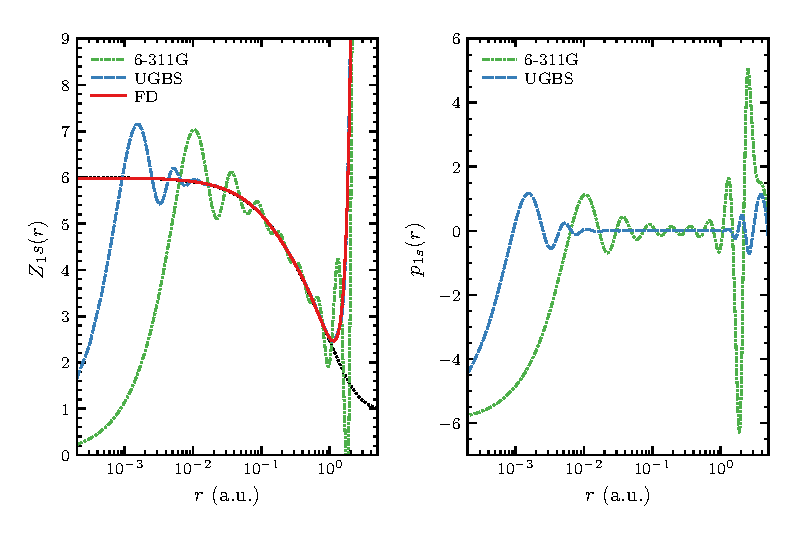
\includegraphics[width=0.9\textwidth]{dim/carbon_prof.eps}
\caption[Inversión de funciones de onda descritas con conjuntos de base.]
{(a) Cargas efectivas invertidas del orbital $1s$ del átomo de carbón.
(b)~Perfiles de oscilación de los conjuntos de base.}
\label{fig:1sCarbon}
\end{figure}

Los patrones de oscilación varían según el conjunto de base utilizado
para representar las soluciones. Definimos los perfiles de oscilación
de cada BS como
\begin{equation}
 p_{nl}^{\mbox{\scriptsize BS}} = Z_{nl}^{\mbox{\scriptsize BS}}-
 Z_{nl}^{\mbox{\scriptsize FD}} \,,
 \label{eq:oscillation-prof}
\end{equation}
donde $Z_{nl}^{\mbox{\scriptsize BS}}$ es la carga invertida del átomo
cuando se usa el conjunto de bases ``BS'' y 
$Z_{nl}^{\mbox{\scriptsize FD}}$ es la carga efectiva que se obtiene a 
partir de la inversión de las soluciones del método de diferencias 
finitas. En el caso del carbono, los conjuntos de base consideradas para 
calcular el orbital $1s$ fueron \mbox{6-311G} y UGBS. Los perfiles de 
oscilación correspondientes a dicho orbital, usando la 
Ec.~(\ref{eq:oscillation-prof}), se muestran en la 
Fig.~\ref{fig:1sCarbon}(b). Dado que los perfiles de oscilación para 
cada conjunto de base atómico son característicos, una vez determinados, 
éstos pueden ser implementados para remover las oscilaciones de los 
cálculos moleculares. 

Una vez que las oscilaciones son removidas de los cálculos moleculares, 
se procede a implentar el procedimiento de depuración descrito en la
Sección~\ref{subsec:depuracion}. Debido a la estructura de las moléculas 
consideras, definimos una nueva ecuación parámetrica para las cargas 
moleculares DIM,
\begin{eqnarray}
 Z(r) = \sum_j z_j e^{-\alpha_j r} 
 + z_{\mbox{\scriptsize H}} e^{-(\ln r - \ln \beta)^2/(2\gamma)} 
 + 1\,.
 \label{eq:molzDIM}
\end{eqnarray}
En constraste con la aproximación propuesta para los 
átomos~(\ref{eq:atomzDIM}), incluimos un segundo término en la fórmula 
analítica de la carga por cuenta de $V_H(r)$, dado 
por~(\ref{eq:Vhidrogenos}). Esta expresión nos permite ajustar 
convenientemente tanto la ubicación como el ancho de los potenciales 
hidrogénicos apantallados sin afectar el valor correcto de la carga en 
el origen.

%%%%%%%%%%%%%%%%%%%%%%%%%%%%%%%%%%%%%%%%%%%%%%%%%%%%%%%%%%%%%%%%%%%%%%%%
\subsection{Potenciales de intercambio}
%%%%%%%%%%%%%%%%%%%%%%%%%%%%%%%%%%%%%%%%%%%%%%%%%%%%%%%%%%%%%%%%%%%%%%%%
\label{subsec:exchpot}

La teoría de Hartree--Fock no incluye términos de correlación en su 
formalismo; así, nuestro método de inversión permite obtener potenciales
de intercambio ``exactos'' $V_{nl}^{\mathrm{DIMx}}(r)$ para cada orbital
$nl$ 
\begin{equation}
V_{nl}^{\mathrm{DIMx}}(r)=V_{nl}^{\mathrm{DIM}}(r)+\frac{Z_{N}}{r}
-\int{ \frac{\rho^{\mathrm{HF}}(r^{\prime})  }
{\left| \mathbf{r} - \mathbf{r^{\prime}} \right|}} \, 
d \mathbf{r^{\prime}} \, ,
\label{eq:exchange-potential}
\end{equation}
donde $\rho^{\mathrm{HF}}(r)$ es la densidad electrónica total que se
calcula a partir de los orbitales HF, $u^{\mathrm{HF}}_{nl}$.

Por supuesto, los potenciales de intercambio orbitales se pueden obtener 
de forma exacta calculando el operador de intercambio de Fock. Sin 
embargo, estos valores son dificiles de expresar mediante expresiones 
simples tales como la Ec.~(\ref{eq:atomzDIM}) debido a la presencia de 
nodos y divergencias que se examinaron previamente. 

An exact average exchange potential can be calculated through the 
average exchange charge density proposed by Slater\cite{Slater:51},
\begin{equation}
 V_{\mathrm{S}}^{\mathrm{x}}(r) = \frac{1}{\rho(r)} \sum_i\sum_j \int 
                       \frac{u_i^*(r)u_j^*(r') u_j(r)u_i(r')}{|\mathbf{r}-
                       \mathbf{r}'|}d\mathbf{r}'\,.
\end{equation}
Our approach, on the other hand, allows us to obtain 
orbital--specific singularity--free exchange potentials 
straigthfowardly.

La energía de intercambio total $E^{\mathrm{x}}$ también se puede 
computar en términos del potencial de intercambio DIM a partir de 
\begin{equation}
E^{\mathrm{x}} = \sum_{nl}E_{nl}^{\mathrm{x}} = 
\sum_{nl}\left[\frac{1}{2}\int{\rho^{\mathrm{HF}}_{nl}(r) \, \, 
V_{nl}^{\mathrm{DIMx}}}(r) \, dr \, \right]
\label{eq:total-energy}
\end{equation}

%%%%%%%%%%%%%%%%%%%%%%%%%%%%%%%%%%%%%%%%%%%%%%%%%%%%%%%%%%%%%%%%%%%%%%%%
\section{Resultados}
%%%%%%%%%%%%%%%%%%%%%%%%%%%%%%%%%%%%%%%%%%%%%%%%%%%%%%%%%%%%%%%%%%%%%%%%
\label{sec:dimresultados}

En esta Sección examinamos los resultados obtenidos a partir de la 
implementación de nuestro método de potencial efectivo para la 
descripción de blancos atómicos y moleculares. La aplicabilidad del 
método de inversión depurada en blancos de estructura compleja es 
evaluada a través del estudio de la ionización por impacto de protones y 
fotones en átomos y moléculas. Analizaremos el desempeño de los  
potenciales DIM ante la primera aproximación de Born para predecir 
secciones eficaces totales de ionización de helio, nitrógeno, neón y 
metano.

%%%%%%%%%%%%%%%%%%%%%%%%%%%%%%%%%%%%%%%%%%%%%%%%%%%%%%%%%%%%%%%%%%%%%%%%
\subsection{Estructura electrónica de blancos}
%%%%%%%%%%%%%%%%%%%%%%%%%%%%%%%%%%%%%%%%%%%%%%%%%%%%%%%%%%%%%%%%%%%%%%%%
\label{subsec:dimtarget}

%%%%%%%%%%%%%%%%%%%%%%%%%%%%%%%%%%%%%%%%%%%%%%%%%%%%%%%%%%%%%%%%%%%%%%%%
\subsubsection*{Helio}
%%%%%%%%%%%%%%%%%%%%%%%%%%%%%%%%%%%%%%%%%%%%%%%%%%%%%%%%%%%%%%%%%%%%%%%%

En primer lugar, mostraremos los resultados obtenidos de implementar
el método de inversión depurada en el átomo de helio en su estado
fundamental. Dado que el orbital $1s$ no tiene nodos y que éste 
decae exponencialmente con la energía del orbital HOMO, la inversión 
directa de este orbital no presenta ninguna de las complicaciones 
numéricas presentadas en la Sección~\ref{subsec:probinv}. Además, la 
simpleza del átomo de helio nos permite ajustar la carga invertida con 
un número reducido de parámetros. Así, es posible optimizar la carga 
efectiva $Z_{1s}^{\mathrm{ DIM}}$, dada por la Ec.~(\ref{eq:atomzDIM}), 
con sólo tres parámetros, los cuales se dan en la 
Tabla~\ref{tab:params-atoms}.

\begin{figure}[t]
\centering
\includegraphics[width=0.9\textwidth]{figures/dim/Hepots.eps}
\caption[Cargas efectivas y potencial de intercambio DIM de He.]
{(a) Cargas efectivas $1s$ del He ($^1$S) obtenidas mediante inversión 
directa (línea discontinua) e inversión depurada (línea sólida). 
(b) Potencial de intercambio DIM (línea sólida) y OPM (línea punteada).}
\label{fig:Hepots}
\end{figure}

Para verificar la calidad de la estructura atómica dada por el potencial 
DIM obtenido, en la Tabla~\ref{tab:results-atoms} presentamos una 
comparación entre los valores de energías y radios medios obtenidos 
utilizando el método de inversión depurada con sus correspondientes 
valores obtenidos mediante el método de Hartree--Fock. El potencial 
$V_{1s}^{\mathrm{ DIM}}$ es capaz de producir un orbital 
$u_{1s}^{\mathrm{ DIM}}$ cuya energía coincide con la energía original 
de HF en 6 cifras significativas. Los valores medios también muestran 
una excelente concordancia, tanto para la región cercana al origen, 
$\langle r \rangle$, como en los que muestrean la calidad de la región 
asintótica, $\langle 1/r\rangle$.


Los valores OPM se obtienen a partir del código \textsc{atomopm} de 
Talman~\cite{Talman:89}.

%%%%%%%%%%%%%% RESULTADOS %%%%%%%%%%%%%%
\begin{table}
\begin{center}
\begin{tabularx}{\textwidth}{
>{\centering\arraybackslash}p{0.12\textwidth}
>{\centering\arraybackslash}p{0.05\textwidth}
>{\centering\arraybackslash}p{0.22\textwidth}
>{\centering\arraybackslash}p{0.22\textwidth}
>{\centering\arraybackslash}p{0.22\textwidth}}
\rowcolor{mydarkgray} 
   &       & $nl$ & $z$        & $\alpha$   \\
%%%%%%%%%%%%%%%%%%%% Helio %%%%%%%%%%%%%%%%%%%%
He & $^1$S & $1s$ &  $1.3175$ & $2.5003$  \\\rowcolor{mygray} 
   &       &      & $-0.3175$ & $5.0437$  \\ 
%%%%%%%%%%%%%%%%%% Nitrogeno %%%%%%%%%%%%%%%%%%
N  & $^4$S & $1s$ & $5.2563$ & $1.2621$  \\\rowcolor{mygray} 
   &       &      & $0.7437$ & $8.0284$  \\ 
   &       & $2s$ & $2.7136$ & $0.8947$ \\\rowcolor{mygray} 
   &       &      & $2.4528$ & $3.5127$  \\
   &       &      & $0.8336$ & $3.3865$  \\ \rowcolor{mygray} 
   &       & $2p$ & $3.6435$ & $1.2407$  \\ 
   &       &      & $2.0550$ & $5.3514$  \\\rowcolor{mygray} 
   &       &      & $0.3015$ & $0.2866$ \\
   & $^2$D & $1s$ & $5.1664$ & $1.2241$  \\\rowcolor{mygray} 
   &       &      & $0.8137$ & $7.5680$  \\ 
   &       & $2s$ & $3.7478$ & $2.8531$  \\\rowcolor{mygray} 
   &       &      & $1.8541$ & $1.0311$  \\ 
   &       &      & $0.3981$ & $0.2397$ \\\rowcolor{mygray} 
   &       & $2p$ & $4.0105$ & $1.2874$  \\ 
   &       &      & $1.8552$ & $5.7086$  \\\rowcolor{mygray} 
   &       &      & $0.1343$ & $0.2680$ \\
   & $^2$P & $1s$ & $5.1864$ & $1.2178$  \\\rowcolor{mygray} 
   &       &      & $0.8137$ & $7.5674$  \\ 
   &       & $2s$ & $3.6700$ & $3.1495$  \\\rowcolor{mygray} 
   &       &      & $1.4394$ & $0.7404$  \\ 
   &       &      & $0.8907$ & $0.8306$ \\\rowcolor{mygray} 
   &       & $2p$ & $2.3280$ & $1.4093$  \\ 
   &       &      & $1.8977$ & $1.1656$  \\\rowcolor{mygray} 
   &       &      & $1.7743$ & $5.6878$ \\
%%%%%%%%%%%%%%%%%%%%%%%%%%%%%%%%%%%%%%%%%%%%%%%
Ne & $^1$S & $1s$ & $7.3677$ & $2.4173$ \\\rowcolor{mygray} 
   &       &      & $1.3004$ & $0.1264$ \\
   &       &      & $0.3320$ & $13.1582$ \\\rowcolor{mygray} 
   &       & $2s$ & $0.2977$ & $17.9939$ \\
   &       &      & $0.6681$ & $0.0673$ \\\rowcolor{mygray} 
   &       &      & $8.0342$ & $2.4722$ \\
   &       & $2p$ & $1.3531$ & $8.5695$ \\\rowcolor{mygray} 
   &       &      & $0.3359$ & $0.4649$ \\
   &       &      & $7.3111$ & $2.0906$ \\
\end{tabularx}
\caption[Parámetros de la carga efectiva de He, N y Ne.]
{Parámetros de la carga efectiva $Z_{1s}^{\mathrm{ DIM}}$ de He ($^1$S), 
N ($^4$S, $^2$D, $^2$P) y Ne ($^1$S).}
\label{tab:params-atoms}
\end{center}
\end{table}

\begin{table}
\begin{center}
\begin{tabularx}{\textwidth}{
>{\centering\arraybackslash}p{0.07\textwidth}
>{\centering\arraybackslash}p{0.03\textwidth}
>{\centering\arraybackslash}p{0.15\textwidth}
>{\centering\arraybackslash}p{0.10\textwidth}
>{\centering\arraybackslash}p{0.15\textwidth}
>{\centering\arraybackslash}p{0.15\textwidth}
>{\centering\arraybackslash}p{0.15\textwidth}}
\rowcolor{mydarkgray} 
   & & $E$ & $nl$ & $\varepsilon_{nl}$ & $\left<r\right>$ & $\left<1/r\right>$ \\
He & $^1$S & $-2.8616$   & $1s$ & $-0.9180$  & $0.9273$ & $1.6873$ \\\rowcolor{mygray} 
   &       & $-2.8617$   &      & $-0.9180$  & $0.9273$ & $1.6873$ \\
N  & $^4$S & $-54.3762$  & $1s$ & $-15.6291$ & $0.2283$ & $6.6487$ \\\rowcolor{mygray} 
   &       & $-54.4009$  &      & $-15.6291$ & $0.2283$ & $6.6532$ \\
   &       &             & $2s$ & $-0.9453$  & $1.3345$ & $1.0804$ \\\rowcolor{mygray} 
   &       &             &      & $-0.9453$  & $1.3323$ & $1.0782$ \\
   &       &             & $2p$ & $-0.5676$  & $1.4127$ & $0.9550$ \\\rowcolor{mygray} 
   &       &             &      & $-0.5676$  & $1.4096$ & $0.9577$ \\
   & $^2$D & $-54.2756$  & $1s$ & $-15.6664$ & $0.2283$ & $6.6493$ \\\rowcolor{mygray} 
   &       & $-54.2962$  &      & $-15.6664$ & $0.2283$ & $6.6539$ \\
   &       &             & $2s$ & $-0.9637$  & $1.3292$ & $1.0874$ \\\rowcolor{mygray} 
   &       &             &      & $-0.9637$  & $1.3263$ & $1.0832$ \\
   &       &             & $2p$ & $-0.5087$  & $1.4488$ & $0.9388$ \\\rowcolor{mygray} 
   &       &             &      & $-0.5087$  & $1.4466$ & $0.9421$ \\
   & $^2$P & $-54.2086$  & $1s$ & $-15.6916$ & $0.2282$ & $6.6504$ \\\rowcolor{mygray} 
   &       & $-54.2281$  &      & $-15.6916$ & $0.2282$ & $6.6543$ \\
   &       &             & $2s$ & $-0.9763$  & $1.3256$ & $1.0871$ \\\rowcolor{mygray} 
   &       &             &      & $-0.9763$  & $1.3223$ & $1.0866$ \\
   &       &             & $2p$ & $-0.4713$  & $1.4718$ & $0.9298$ \\\rowcolor{mygray} 
   &       &             &      & $-0.4713$  & $1.4730$ & $0.9316$ \\
Ne & $^1$S & $-128.4978$ & $1s$ & $-32.7725$ & $0.1575$ & $9.6215$ \\\rowcolor{mygray} 
   &       & $-128.5475$ &      & $-32.7724$ & $0.1576$ & $9.6181$ \\
   &       &             & $2s$ & $-1.9304$  & $0.8913$ & $1.6408$ \\\rowcolor{mygray} 
   &       &             &      & $-1.9304$  & $0.8921$ & $1.6326$ \\  
   &       &             & $2p$ & $-0.8504$  & $0.9678$ & $1.4303$ \\\rowcolor{mygray} 
   &       &             &      & $-0.8504$  & $0.9653$ & $1.4354$ \\
\end{tabularx}
\caption[Energías y radios medios de He, N y Ne.]
{Energías totales, radios medios y energías orbitales obtenidos con el 
método de inversión depurada (filas superiores) y con el método de HF 
(filas inferiores) de He ($^1$S), N ($^4$S, $^2$D, $^2$P) y Ne ($^1$S).}
\label{tab:results-atoms}
\end{center}
\end{table}

\begin{figure}[t]
\centering
\includegraphics[width=0.9\textwidth]{figures/dim/N4S_DIM.eps}
\caption[Cargas efectivas DIM de N.]
{Cargas efectivas $1s$, $2s$ y $2p$ del término $^4$S de N obtenidas 
mediante inversión directa (lineas discontinuas) e inversión depurada 
(líneas sólidas).}
\label{fig:Nzeff}
\end{figure}

\begin{table}
\begin{center}
\begin{tabularx}{\textwidth}{
>{\centering\arraybackslash}p{0.07\textwidth}
>{\centering\arraybackslash}p{0.03\textwidth}
>{\centering\arraybackslash}p{0.14\textwidth}
>{\centering\arraybackslash}p{0.14\textwidth}
>{\centering\arraybackslash}p{0.14\textwidth}
>{\centering\arraybackslash}p{0.14\textwidth}
>{\centering\arraybackslash}p{0.14\textwidth}}
\rowcolor{mydarkgray} 
   &       & $1s$      & $2s$      & $3s$      & Total     & EAHF~\cite{Becke:14} \\
He & $^1$S & $-0.5129$ &           &           & $-1.0258$ & $-1.026$ \\\rowcolor{mygray} 
N  & $^4$S & $-2.1175$ & $-0.4776$ & $-0.4711$ & $-6.6034$ & $-6.596$ \\
   & $^2$D & $-2.1175$ & $-0.4777$ & $-0.4262$ & $-6.4688$ & \\\rowcolor{mygray} 
   & $^2$P & $-2.1175$ & $-0.4780$ & $-0.3973$ & $-6.3827$ & \\
Ne & $^1$S & $-3.1106$ & $-0.8620$ & $-0.6938$ & $-12.1080$ & $-12.11$ \\\rowcolor{mygray} 
%$^{\dagger}$ Ref. 
\end{tabularx}
\caption[Energías de intercambio total y orbitales de He, N y Ne.]
{Energías de intercambio total y orbitales DIM de He ($^1$S), N ($^4$S, 
$^2$D, $^2$P) y Ne ($^1$S).}
\label{tab:results-atoms}
\end{center}
\end{table}


\begin{figure}[t]
\centering
\includegraphics[width=0.9\textwidth]{figures/dim/N_Vx.eps}
\caption[Potenciales de intercambio DIM de N.]
{Potenciales de intercambio DIM de los términos $^4$S (línea sólida), 
$^2$D (línea discontinua) y $^2$P (línea punto-raya), y valores OPM 
(línea punteada) de N.}
\label{fig:NVx}
\end{figure}


%%%%%%%%%%%%%%%%%%%%%%%%%%%%%%%%%%%%%%%%%%%%%%%%%%%%%%%%%%%%%%%%%%%%%%%%
\subsubsection*{Nitrógeno}
%%%%%%%%%%%%%%%%%%%%%%%%%%%%%%%%%%%%%%%%%%%%%%%%%%%%%%%%%%%%%%%%%%%%%%%%

Los excelentes resultados obtenidos a partir de la implementación de DIM 
en el átomo de helio pueden atribuirse a la simplicidad del orbital y su 
simetría esférica. Para evaluar la destreza del método de inversión 
depurada para describir blancos con más electrones y de capa abierta, 
consideramos ahora el átomo de nitrógeno. 

La configuración más baja del nitrógeno $2p^3$ da lugar a tres términos 
diferentes: $^4$S, $^2$D, $^2$P. Cada uno de estos términos está 
descrito por una densidad electrónica diferente. Consideramos aquí 
las soluciones de HF del término de menor energía. En la  
Fig.~\ref{fig:Nzeff} se muestran las cargas de los orbitales $1s$, $2s$ 
y $2p$ obtenidas a partir del método de inversión (líneas discontinuas) 
y el método de inversión depurada (líneas continuas). Como se estudiado 
en la Sección~\ref{subsec:probinv}, la inversión del orbital 
$u_{1s}^{\mathrm{HF}}$ diverge en la región asintótica debido al 
comportamiento del potencial dado por la Ec.~\ref{eq:asintoticoVHF}. 
Además, el nodo genuino del orbital $2s$, en $r\approx 0.32$~a.u., es 
traducido por el método de inversión (IM) como un polo a la carga. 

La implementación del método de inversión depurada permite ajustar 
analíticamente la carga invertida en el mayor rango posible. Luego de 
una optimización cuidadosa del blanco se obtienen los parámetros de las 
cargas DIM correspondientes el término $^4$S que se dan en la 
Tabla~\ref{tab:params-atoms}. Resolviendo la ecuación de Schr\"odinger 
para un electrón (\ref{eq:eqSchroRadial}) con las cargas efectivas DIM 
es posible reproducir las energías orbitales hasta la quinta cifra 
significativa de los valores de Hartree--Fock y los valores medios 
$\langle r \rangle$ y $\langle 1/r \rangle$ hasta en un $0.2\%$, como se 
muestra en la Tabla~\ref{tab:results-atoms}.  


%%%%%%%%%%%%%%%%%%%%%%%%%%%%%%%%%%%%%%%%%%%%%%%%%%%%%%%%%%%%%%%%%%%%%%%%
\subsubsection*{Neón}
%%%%%%%%%%%%%%%%%%%%%%%%%%%%%%%%%%%%%%%%%%%%%%%%%%%%%%%%%%%%%%%%%%%%%%%%

La implementación del DIM en neón es análoga al caso de nitrógeno. Los 
resultados de la optimización de los parámetros que definen las cargas 
efectivas, dadas por la Ec.~(\ref{eq:atomzDIM}), del átomo de neón se 
muestran en la Tabla~\ref{tab:params-atoms}. La comparación entre las 
soluciones de los potenciales DIM y el método de Hartree--Fock se dan en 
la Tabla~\ref{tab:results-atoms}. El acuerdo en energías orbitales es 
excelente, del orden de $1\times 10^{-5}$, mientras que DIM reproduce 
los valores medios de los orbitales HF en aproximadamente $0.1\%$. 

%%%%%%%%%%%%%%%%%%%%%%%%%%%%%%%%%%%%%%%%%%%%%%%%%%%%%%%%%%%%%%%%%%%%%%%%
\subsubsection*{Metano}
%%%%%%%%%%%%%%%%%%%%%%%%%%%%%%%%%%%%%%%%%%%%%%%%%%%%%%%%%%%%%%%%%%%%%%%%

La expansión del método de inversión depurada a sistemas moleculares es 
aplicada a la molécula de metano. Este hidruro es altamente simétrico y, 
por lo tanto, puede ser descrito por un potencial angular  
promediado~\cite{Granados:16}. 

\begin{figure}[t]
\centering
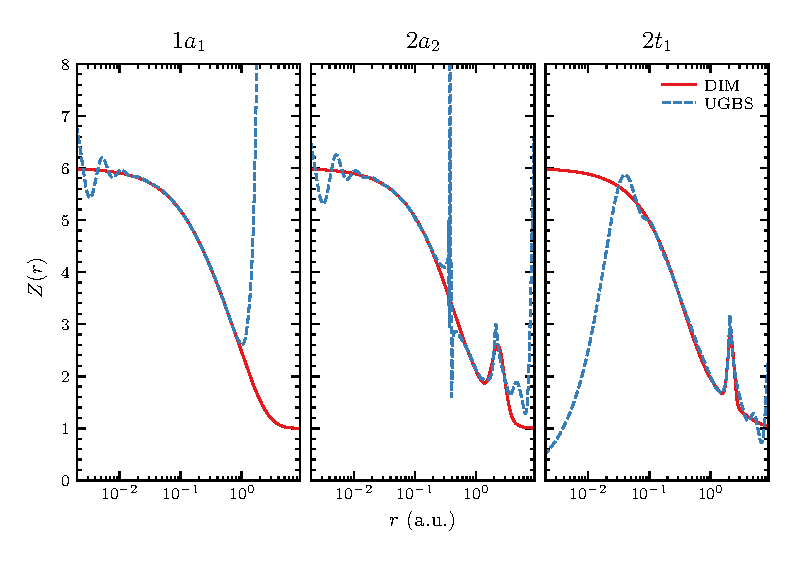
\includegraphics[width=0.9\textwidth]{figures/dim/ch4_dim.eps}
\caption[Cargas efectivas DIM de metano.]
{Cargas efectivas de CH$_4$; inversión directa (lineas discontinuas)
e inversión depurada (líneas sólidas).}
\label{fig:ch4zeff}
\end{figure}

Los orbitales moleculares de HF de CH$_4$ se calcularon usando los 
conjuntos de bases UGBS del carbono y el hidrógeno, los cuales 
consideran momentos angulares hasta $L=1$. El cálculo de estructura 
electrónico de metano con estos conjuntos de base deberían incluir 
funciones de polarización (por lo menos hasta las funciones $d$), con el 
fin de incrementar la precisión de las energías  
moleculares~\cite{Rothenberg:71,Hariharan:72}. Sin embargo, para aislar 
los efectos de los conjuntos de base, realizamos los cálculos de 
perfiles de oscilación descritos en la Sección~\ref{sec:dimmoleculas} y 
los orbitales moleculares en el mismo esquema. Las cargas obtenidas 
mediante la inversión directa se muestran en la Fig.~\ref{fig:ch4zeff} 
con líneas discontinuas. Dado que los orbitales moleculares están 
escritos por combinaciones lineales de orbitales atómicos del carbono y 
el hidrógeno, las oscilaciones de las cargas invertidas se deben al 
número finito de funciones primitivas en el conjunto de base de cada 
átomo. Para remover estas oscilaciones, se deben determinar los perfiles 
de oscilación producidas por el conjunto de base de los átomos 
constituyentes. Usamos la Ec.~(\ref{eq:oscillation-prof}) para 
determinar los perfiles $p_{1s}^{\mbox{\scriptsize UGBS}}$, 
$p_{2s}^{\mbox{\scriptsize UGBS}}$ y $p_{2p}^{\mbox{\scriptsize UGBS}}$ 
del carbono. Así, se puden remover los perfiles 
$p_{nl}^{\mbox{\scriptsize UGBS}}$ de las correspondientes cargas 
invertidas $Z_{i}^{\mbox{\scriptsize UGBS}}$ del metano. Las 
oscilaciones se remueven completamente para todos los orbitales excepto 
el $2a_2$, que presenta pequeñas fluctuaciones residuales debido a la 
base del hidrógeno. Ya que estas ondulaciones son mínimas y se ubican 
cerca del núcleo, podemos despreciarlas y procedemos a implementar le 
método de depuración descrita en la Sección~\ref{sec:dimmoleculas}. 

Los parámetros optimizados de las cargas moleculares DIM, dadas por la 
Ec.~(\ref{eq:molzDIM}), se dan en la Tabla~\ref{tab:ch4parameters}. Las 
cargas correspondientes se muestran en la Fig.~\ref{fig:ch4zeff} con 
líneas sólidas.  En este caso, para la construcción de función de 
costo~(\ref{eq:fncosto-dim}) minimizada se consideraron los valores de 
energía y los valores medios de los MOs dados por 
Moccia~\cite{Moccia:69}. Los valores de energía obtenidos con ellas 
reproducen las originales hasta la cuarta cifra significativa y se dan 
en la Tabla~\ref{tab:ch4parameters}. Por otro lado, los valores medios 
$\langle r\rangle$ y $\langle 1/r\rangle$ obtenidos con los potenciales 
moleculares DIM son en promedio del $0.3\%$ y menores al $1\%$.

\begin{table}[t]
\centering
\begin{tabular}{
>{\centering\arraybackslash}p{0.13\textwidth}
>{\centering\arraybackslash}p{0.13\textwidth}
>{\centering\arraybackslash}p{0.13\textwidth}
>{\centering\arraybackslash}p{0.13\textwidth}
>{\centering\arraybackslash}p{0.13\textwidth}
>{\centering\arraybackslash}p{0.13\textwidth}}
\rowcolor{mydarkgray} 
   $nl$ & $E$        & $z$        & $\alpha$   & $\beta$ & $\gamma$ \\
$1a_1$  & $-11.1949$ & $1.925280$ & $0.641982$ & & \\
\rowcolor{mygray} 
        &            & $0.953120$ & $5.571510$ & & \\
        &            & $2.121600$ & $1.500440$ & & \\
\rowcolor{mygray} 
$2a_2$  & $-0.9204$  & $2.912200$ & $3.149990$ & & \\
        &            & $2.087800$ & $0.771371$ & & \\
\rowcolor{mygray} 
        &            & $1.23640$  &            & $2.329570$ & $0.053420$ \\
$2t_1$  & $-0.5042$  & $0.901953$ & $2.895140$ & & \\
\rowcolor{mygray} 
        &            & $1.112030$ & $0.388649$ & & \\
        &            & $2.986017$ & $2.931210$ & & \\
\rowcolor{mygray} 
        &            & $1.301820$ &            & $2.169850$ & $0.012616$ \\ 
\end{tabular}
\caption[Energías y parámetros de ajuste de cargas efectivas de metano.]
{Energías orbitales moleculares y parámetros de ajuste de cargas efectivas dadas por la Ec.~(\ref{eq:molzDIM}) de metano.}
\label{tab:ch4parameters}
\end{table}

%%%%%%%%%%%%%%%%%%%%%%%%%%%%%%%%%%%%%%%%%%%%%%%%%%%%%%%%%%%%%%%%%%%%%%%%
\subsection{Procesos colisionales simples}
%%%%%%%%%%%%%%%%%%%%%%%%%%%%%%%%%%%%%%%%%%%%%%%%%%%%%%%%%%%%%%%%%%%%%%%%

En esta Sección analizaremos la respuesta del potencial efectivo DIM, 
obtenido mediante el método de inversión depurada, para describir la 
estructura de blancos atómicos y molecular en el proceso de 
fotoionización de tres blancos atómicos --helio, nitrógeno y neón-- y un 
blanco molecular simple: metano. La estructura de los blancos, con 
estado de carga neutro y en sus estados fundamentales de menor energía, 
está dada por los resultados de la Sección~\ref{subsec:dimtarget}. 
En los blancos moleculares, la orientación molecular es importante para 
determinar la sección eficaz en un proceso colisional. Sin embargo, en 
sistemas gasesosos, las moléculas tienen orientaciones aleatorias que no 
están predefinidas en el experimento. Por lo tanto, la descripción 
promediada esféricamente de los sistemas moleculares asumida por el 
potencial DIM está en concordancia con la configuración del blanco.
Los procesos colisionales examinados en esta Sección se describen a 
primer orden empleando la primera aproximación de Born (FBA). 
Denominamos la combinación de la descripción del blanco mediante el 
potencial efectivo DIM y el modelado de la fotoionización a primer orden 
como fotoionización DIM-FBA.  

%%%%%%%%%%%%%%%%%%%%%%%%%%%%%%%%%%%%%%%%%%%%%%%%%%%%%%%%%%%%%%%%%%%%%%%%
\subsubsection{Fotoionización}
%%%%%%%%%%%%%%%%%%%%%%%%%%%%%%%%%%%%%%%%%%%%%%%%%%%%%%%%%%%%%%%%%%%%%%%%
\label{subsec:foto}

Las secciones eficaces de ionización simple por impacto de fotón según 
el modelo DIM-FBA para helio, nitrógeno, neón y metano se muestran en 
la Fig.~\ref{fig:photoDIM} con líneas 
sólidas. Los resultados teóricos DIM-FBA para helio y nitrógeno 
coinciden de manera excelente con los valores experimentales 
(símbolos)~\cite{Samson:90,Henke:93,Stolte:16} a bajas, medias y altas 
energías del fotón incidente. En el caso del átomo de neón, algunas 
discrepancias con las mediciones (símbolos) \cite{Henke:93,Samson:02} 
empiezan a surgir a energías bajas e intermedias del projectil. Este 
comportamiento sugiere la necesidad de incluir en la descripción de la 
fotoionización correcciones de mayor orden que incluyan efectos de 
múltiples cuerpos que puedan ser relevantes tales como la relajación de 
los orbitales debido a la creación de un hueco electrónico, respuestas 
colectivas de electrones de capas internas~\cite{Ederer:64} y efectos de 
correlación.

\begin{figure}
\centering
\includegraphics[width=0.92\textwidth]{dim/fotoDIM-part1.eps} 

\vspace{-1.15cm}
\includegraphics[width=0.92\textwidth]{dim/fotoDIM-part2.eps}
\caption[Fotoionización de He, N, Ne y CH$_4$.]
{Sección eficaz total de fotoionización de un electrón de He~$^1$S, 
N~$^4$S, Ne~$^1$S y CH$_4$. Curvas: cálculos teóricos DIM-FBA. Símbolos: 
datos experimentales~\cite{Samson:90,Henke:93,Stolte:16,Samson:02,
Lukirskii:64,Henke:82,Samson:89}.}
\label{fig:photoDIM}
\end{figure}

La predicción del modelo DIM-FBA para la sección eficaz total de 
fotonización de CH$_4$ se encuentra en buen acuerdo con valores 
experimentales en el rango de altas energías y cerca del umbral. La 
curva entre aproximadamente 15 y 300 eV muestra la fotoionización de la 
capa eterna $n=2$, mientras que la discontinuidad en $0.3$~keV 
corresponde al umbral del orbital molecular $1a_1$. Para fotoenergías 
bajas e intermedias, el acuerdo entre nuestras predicciones y los datos 
experimentales~\cite{Lukirskii:64,Henke:82,Samson:89} no es bueno. 
Fenónemos tales como la relajación de los orbitales moleculares, 
posibles contribuciones colectivas y efectos de correlación deben ser  
considerados en futuros cálculos. Por otro lado, para la fotoionización 
de un electrón perteneciente al orbital interno $1a_1$, estos efectos no 
son tan signficativos, y obtenemos buen acuerdo con los valores 
experimentales disponibles. 

%=======================================================================
\subsubsection{Ionización por impacto de iones}
\label{subsec:dimion}

\begin{figure}
\centering
\includegraphics[width=0.9\textwidth]{figures/dim/ionDIM.eps}
\caption[Ionización por impacto de protón de N y CH$_4$.]
{Sección eficaz total de ionización de un electrón por impacto de protón 
de N~$^4$S y CH$_4$. Línea sólida: cálculos teóricos DIM-FBA. 
Símbolos: datos experimentales de ionización por impacto de 
protón~\cite{Rudd:83,Rudd:85} y electrón~\cite{Brook:78} con conversión 
de equivelocidad.}
\label{fig:iondim}
\end{figure}

Los resultados de ionización por impacto de protón en N~$^4$S y CH$_4$, 
en el marco del modelo DIM-FBA, se muestra en la Fig.~\ref{fig:iondim}. 
El acuerdo entre nuestras predicciones teóricas y las datos 
experimentales es muy bueno en la región de altas energías, donde tiene 
validez la primera aproximación de Born. En el caso de nitrógeno, 
incluimos también datos experimentales de ionización por impacto de 
electrón. Para valores de energía mayores a 400~keV, se espera que la 
sección eficaz de ambos proyectiles coincida. 

%=======================================================================
\section{Conclusiones}
\label{conclusion}

En este Capítulo desarrollamos el método de inversión depurada (DIM) 
para obtener potenciales efectivos que permitan describir la estructura 
electrónica de blancos atómicos y moleculares de manera precisa. La 
disponibilidad de estos potenciales permite conocer los estados 
iniciales y finales del blanco en una colisión de manera directa. 

Los potenciales DIM se obtienen a partir de la inversión de ecuaciones 
de un electrón con soluciones de Hartree--Fock. Los potenciales 
resultantes presentan defectos numéricos (polos y divergencias), los 
cuales son examinados en detalle. Encontramos que el origen de estos 
defectos se ubica en la teoría de Hartree--Fock. Los polos se deben a 
que los nodos genuinos de los orbitales HF no son puntos de inflexión. 
Si bien esta característica de los orbitales no es explícita en la 
teoría, la obtención de potenciales sin polos así lo requiere. Las 
divergencias asintóticas del potencial se deben al coeficiente del 
decaimiento exponencial de los orbitales HF. La teoría de HF establece 
que éstos decaen con la energía del HOMO. Sin embargo, la obtención de 
potenciales con correcto comportamiento asintótico mediante el esquema 
de inversión requiere que cada orbital decaiga con la energía del dicho 
orbital. También se encontraron oscilaciones en los orbitales de las 
capas internas de átomos con carga nuclear $Z\ge 12$, que dan lugar a  
nodos espúreos. Es posible que estas oscilaciones se deban al término de 
intercambio a grandes distancias. Para tratar los defectos encontrados 
en la inversión, se desarrolló el método de depuración, que consiste en 
ajustar las cargas invertidas, en regiones sin polos ni divergencias, 
mediante una expresión analítica. Los parámetros que definen esta 
expresión son optimizados cuidadosamente hasta reproducir las soluciones 
iniciales.

El método de inversión depurada para átomos fue extendido para 
moléculas. Debido a que los orbitales moleculares se expresan a partir 
de conjuntos de base finitas, las soluciones presentan ondulaciones casi 
imperceptiles. La implementación de la inversión traduce estas pequeñas 
fluctuaciones como grandes oscilaciones en la carga molecular. Debido a 
esto, se requieren pasos adicionales en el método de depuración, los 
cuales incluyen la determinación de perfiles de oscilación de los 
conjuntos de base atómicas utilizadas en el cálculo molecular. 

Implementamos el método DIM para obtener potenciales efectivos que 
reproducen las soluciones de HF de forma precisa en tres blancos 
atómicos --helio, nitrógeno y neón-- y un sistema molecular de simetría 
esférica: metano. La efectividad del DIM para describir la estructura de 
blancos en una colisión fue examinado a partir de la primera 
aproximación de Born. Los potenciales de He, N, Ne y CH$_4$ se 
implementaron para calcular, en conjunción con la FBA, secciones 
eficaces de ionización por el impacto de protones y fotones. Ambos 
procesos son reproducidos en términos generales con buena concordancia 
con los datos experimentales disponibles. Las discrepancias principales 
se atribuyen al hecho de que nuestro cálculo sólo considera el primer 
orden perturbativo. Será necesario implementar métodos perturbativos con 
mayor orden de aproximación para examinar la validez del método DIM en 
la región de energías intermedias.





